\documentclass{standalone}
\usepackage{tikz}
\usetikzlibrary{patterns, positioning}
\usepackage[sfdefault]{ClearSans} %% option 'sfdefault' activates Clear Sans as the default text font
\usepackage[T1]{fontenc}

\begin{document}
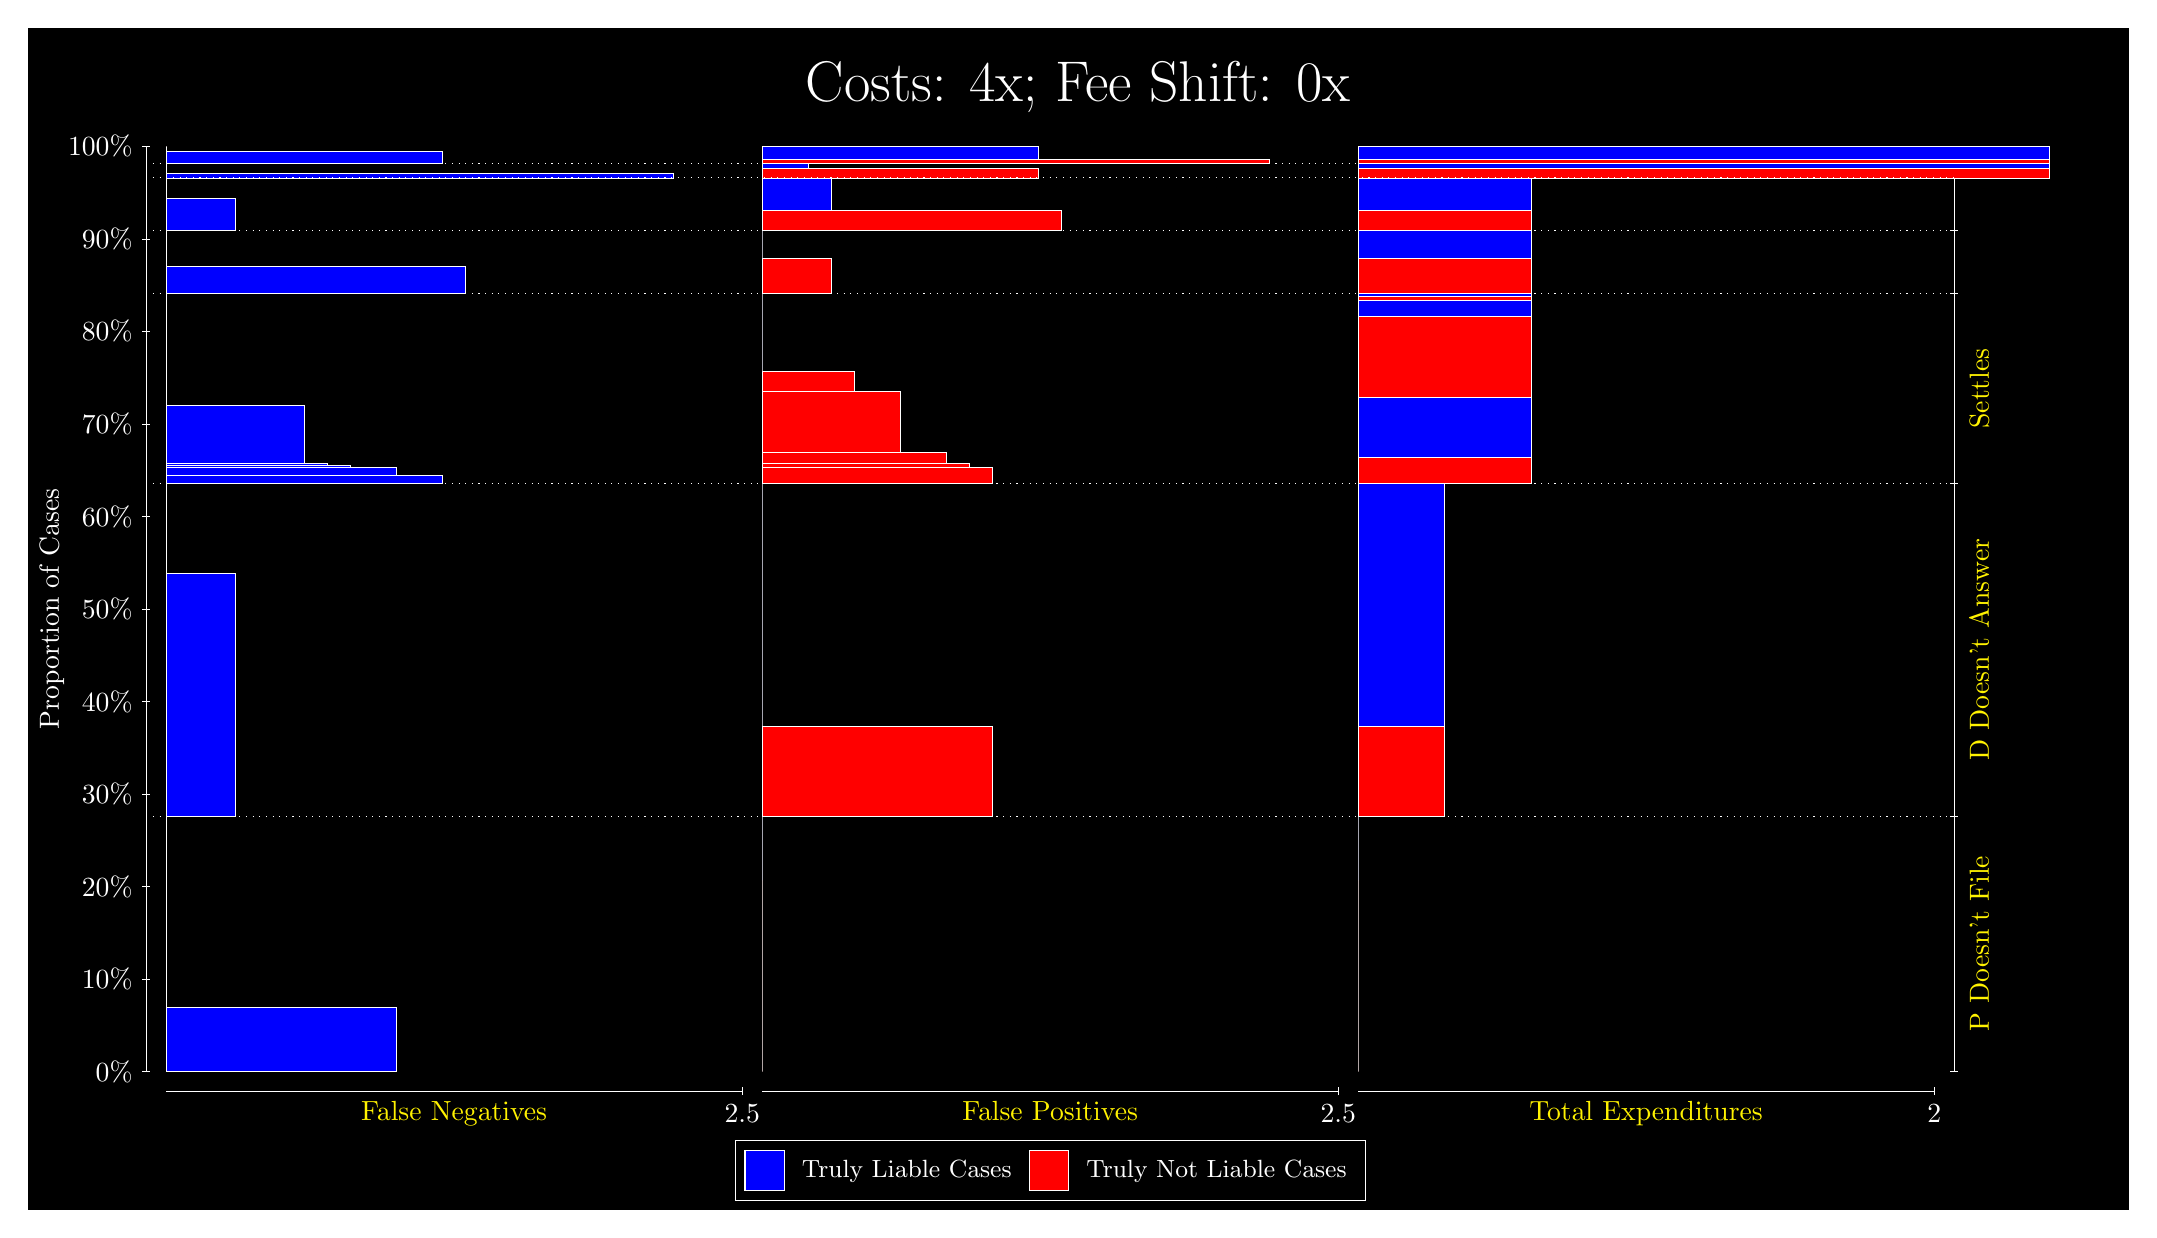
\begin{tikzpicture}
\draw[fill=black] (0,0) rectangle (26.667,15);
\draw[text=white] (0,13.5) rectangle (26.667,15) node[midway] {\huge Costs: 4x; Fee Shift: 0x};
\draw[white, very thin] (1.5,1.75) -- (1.5,13.5);
\node[rotate=90, text=white, anchor=center] at (0.3, 7.625) {Proportion of Cases};
\draw[white, very thin] (1.45,1.75) -- (1.55,1.75);
\node[text=white, anchor=east] at (1.45, 1.75) {0\%};
\draw[white, very thin] (1.45,2.925) -- (1.55,2.925);
\node[text=white, anchor=east] at (1.45, 2.925) {10\%};
\draw[white, very thin] (1.45,4.1) -- (1.55,4.1);
\node[text=white, anchor=east] at (1.45, 4.1) {20\%};
\draw[white, very thin] (1.45,5.275) -- (1.55,5.275);
\node[text=white, anchor=east] at (1.45, 5.275) {30\%};
\draw[white, very thin] (1.45,6.45) -- (1.55,6.45);
\node[text=white, anchor=east] at (1.45, 6.45) {40\%};
\draw[white, very thin] (1.45,7.625) -- (1.55,7.625);
\node[text=white, anchor=east] at (1.45, 7.625) {50\%};
\draw[white, very thin] (1.45,8.8) -- (1.55,8.8);
\node[text=white, anchor=east] at (1.45, 8.8) {60\%};
\draw[white, very thin] (1.45,9.975) -- (1.55,9.975);
\node[text=white, anchor=east] at (1.45, 9.975) {70\%};
\draw[white, very thin] (1.45,11.15) -- (1.55,11.15);
\node[text=white, anchor=east] at (1.45, 11.15) {80\%};
\draw[white, very thin] (1.45,12.325) -- (1.55,12.325);
\node[text=white, anchor=east] at (1.45, 12.325) {90\%};
\draw[white, very thin] (1.45,13.5) -- (1.55,13.5);
\node[text=white, anchor=east] at (1.45, 13.5) {100\%};

\draw[white, very thin] (24.457,1.75) -- (24.457,13.5);
\draw[white, very thin] (24.407,1.75) -- (24.507,1.75);
\node[anchor=west] at (24.407, 1.75) {};
\draw[white, very thin] (24.407,4.9943) -- (24.507,4.9943);
\node[anchor=west] at (24.407, 4.9943) {};
\draw[white, very thin] (24.407,9.2199) -- (24.507,9.2199);
\node[anchor=west] at (24.407, 9.2199) {};
\draw[white, very thin] (24.407,11.629) -- (24.507,11.629);
\node[anchor=west] at (24.407, 11.629) {};
\draw[white, very thin] (24.407,12.428) -- (24.507,12.428);
\node[anchor=west] at (24.407, 12.428) {};
\draw[white, very thin] (24.407,13.1) -- (24.507,13.1);
\node[anchor=west] at (24.407, 13.1) {};
\draw[white, very thin] (24.407,13.282) -- (24.507,13.282);
\node[anchor=west] at (24.407, 13.282) {};
\draw[white, very thin] (24.407,13.5) -- (24.507,13.5);
\node[anchor=west] at (24.407, 13.5) {};

\draw[white, very thin, fill=blue] (1.75,1.75) rectangle (4.6775,2.5648);
\draw[white, very thin, fill=red] (1.75,2.5648) rectangle (1.75,4.9943);
\draw[white, very thin, fill=blue] (1.75,4.9943) rectangle (2.6283,8.0783);
\draw[white, very thin, fill=red] (1.75,8.0783) rectangle (1.75,9.2199);
\draw[white, very thin, fill=blue] (1.75,9.2199) rectangle (5.2631,9.3251);
\draw[white, very thin, fill=blue] (1.75,9.3251) rectangle (4.6775,9.4226);
\draw[white, very thin, fill=blue] (1.75,9.4226) rectangle (4.092,9.4478);
\draw[white, very thin, fill=blue] (1.75,9.4478) rectangle (3.7993,9.477);
\draw[white, very thin, fill=blue] (1.75,9.477) rectangle (3.5065,10.211);
\draw[white, very thin, fill=red] (1.75,10.211) rectangle (1.75,11.629);
\draw[white, very thin, fill=blue] (1.75,11.629) rectangle (5.5558,11.979);
\draw[white, very thin, fill=red] (1.75,11.979) rectangle (1.75,12.428);
\draw[white, very thin, fill=blue] (1.75,12.428) rectangle (2.6283,12.844);
\draw[white, very thin, fill=red] (1.75,12.844) rectangle (1.75,13.1);
\draw[white, very thin, fill=blue] (1.75,13.1) rectangle (8.1906,13.159);
\draw[white, very thin, fill=red] (1.75,13.159) rectangle (1.75,13.282);
\draw[white, very thin, fill=blue] (1.75,13.282) rectangle (5.2631,13.441);
\draw[white, very thin, fill=red] (1.75,13.441) rectangle (1.75,13.5);
\draw[white, very thin, fill=red] (9.3189,1.75) rectangle (9.3189,4.1795);
\draw[white, very thin, fill=blue] (9.3189,4.1795) rectangle (9.3189,4.9943);
\draw[white, very thin, fill=red] (9.3189,4.9943) rectangle (12.246,6.136);
\draw[white, very thin, fill=blue] (9.3189,6.136) rectangle (9.3189,9.2199);
\draw[white, very thin, fill=red] (9.3189,9.2199) rectangle (12.246,9.4215);
\draw[white, very thin, fill=red] (9.3189,9.4215) rectangle (11.954,9.4741);
\draw[white, very thin, fill=red] (9.3189,9.4741) rectangle (11.661,9.6095);
\draw[white, very thin, fill=red] (9.3189,9.6095) rectangle (11.075,10.385);
\draw[white, very thin, fill=red] (9.3189,10.385) rectangle (10.49,10.638);
\draw[white, very thin, fill=blue] (9.3189,10.638) rectangle (9.3189,11.629);
\draw[white, very thin, fill=red] (9.3189,11.629) rectangle (10.197,12.078);
\draw[white, very thin, fill=blue] (9.3189,12.078) rectangle (9.3189,12.428);
\draw[white, very thin, fill=red] (9.3189,12.428) rectangle (13.125,12.683);
\draw[white, very thin, fill=blue] (9.3189,12.683) rectangle (10.197,13.1);
\draw[white, very thin, fill=red] (9.3189,13.1) rectangle (12.832,13.223);
\draw[white, very thin, fill=blue] (9.3189,13.223) rectangle (9.9044,13.282);
\draw[white, very thin, fill=red] (9.3189,13.282) rectangle (15.759,13.341);
\draw[white, very thin, fill=blue] (9.3189,13.341) rectangle (12.832,13.5);
\draw[white, very thin, fill=red] (16.888,1.75) rectangle (16.888,4.1795);
\draw[white, very thin, fill=blue] (16.888,4.1795) rectangle (16.888,4.9943);
\draw[white, very thin, fill=red] (16.888,4.9943) rectangle (17.986,6.136);
\draw[white, very thin, fill=blue] (16.888,6.136) rectangle (17.986,9.2199);
\draw[white, very thin, fill=red] (16.888,9.2199) rectangle (19.083,9.5569);
\draw[white, very thin, fill=blue] (16.888,9.5569) rectangle (19.083,10.317);
\draw[white, very thin, fill=red] (16.888,10.317) rectangle (19.083,11.345);
\draw[white, very thin, fill=blue] (16.888,11.345) rectangle (19.083,11.548);
\draw[white, very thin, fill=red] (16.888,11.548) rectangle (19.083,11.6);
\draw[white, very thin, fill=blue] (16.888,11.6) rectangle (19.083,11.629);
\draw[white, very thin, fill=red] (16.888,11.629) rectangle (19.083,12.078);
\draw[white, very thin, fill=blue] (16.888,12.078) rectangle (19.083,12.428);
\draw[white, very thin, fill=red] (16.888,12.428) rectangle (19.083,12.683);
\draw[white, very thin, fill=blue] (16.888,12.683) rectangle (19.083,13.1);
\draw[white, very thin, fill=red] (16.888,13.1) rectangle (25.67,13.223);
\draw[white, very thin, fill=blue] (16.888,13.223) rectangle (25.67,13.282);
\draw[white, very thin, fill=red] (16.888,13.282) rectangle (25.67,13.341);
\draw[white, very thin, fill=blue] (16.888,13.341) rectangle (25.67,13.5);
\draw[white, dotted] (1.5,4.9943) -- (24.457,4.9943);
\draw[white, dotted] (1.5,9.2199) -- (24.457,9.2199);
\draw[white, dotted] (1.5,11.629) -- (24.457,11.629);
\draw[white, dotted] (1.5,12.428) -- (24.457,12.428);
\draw[white, dotted] (1.5,13.1) -- (24.457,13.1);
\draw[white, dotted] (1.5,13.282) -- (24.457,13.282);
\draw[white, very thin] (1.75,1.5) -- (9.0689,1.5);
\node[text=yellow, anchor=north] at (5.4094, 1.5) {False Negatives};
\draw[white, very thin] (9.0689,1.45) -- (9.0689,1.55);
\node[text=white, anchor=north] at (9.0689, 1.45) {2.5};

\draw[white, very thin] (9.3189,1.5) -- (16.638,1.5);
\node[text=yellow, anchor=north] at (12.978, 1.5) {False Positives};
\draw[white, very thin] (16.638,1.45) -- (16.638,1.55);
\node[text=white, anchor=north] at (16.638, 1.45) {2.5};

\draw[white, very thin] (16.888,1.5) -- (24.207,1.5);
\node[text=yellow, anchor=north] at (20.547, 1.5) {Total Expenditures};
\draw[white, very thin] (24.207,1.45) -- (24.207,1.55);
\node[text=white, anchor=north] at (24.207, 1.45) {2};

\node[text=yellow, centered, rotate=90] at (24.777, 3.3722) {P Doesn't File};
\node[text=yellow, centered, rotate=90] at (24.777, 7.1071) {D Doesn't Answer};
\node[text=yellow, centered, rotate=90] at (24.777, 10.425) {Settles};





\draw (12.978300999999998,1.5) node[draw=none] (baseCoordinate) {};
\begin{scope}[align=center]
        \matrix[scale=0.5, draw=white, below=0.5cm of baseCoordinate, nodes={draw}, column sep=0.1cm]{
            \node[rectangle, draw, minimum width=0.5cm, minimum height=0.5cm, fill=blue] {}; &
            \node[draw=none, font=\small, text=white] (B) {Truly Liable Cases}; &
            \node[rectangle, draw, minimum width=0.5cm, minimum height=0.5cm, fill=red] {}; &
            \node[draw=none, font=\small, text=white] (B) {Truly Not Liable Cases}; \\
            };
\end{scope}

\end{tikzpicture}
\end{document}